% Options for packages loaded elsewhere
\PassOptionsToPackage{unicode}{hyperref}
\PassOptionsToPackage{hyphens}{url}
%
\documentclass[11pt]{article}
\usepackage{comment}
\usepackage[letterpaper,margin=0.9in]{geometry}
\usepackage{setspace}
\setstretch{1.0}
\setlength{\parindent}{0pt}
\setlength{\parskip}{5pt}
\usepackage{amsmath,amssymb}
\usepackage{iftex}
\ifPDFTeX
  \usepackage[T1]{fontenc}
\usepackage{lmodern}
  \usepackage[utf8]{inputenc}
  \usepackage{textcomp} % provide euro and other symbols
\else % if luatex or xetex
  \usepackage{unicode-math} % this also loads fontspec
  \defaultfontfeatures{Scale=MatchLowercase}
  \defaultfontfeatures[\rmfamily]{Ligatures=TeX,Scale=1}
\fi
\ifPDFTeX\else
  % xetex/luatex font selection
\fi
% Use upquote if available, for straight quotes in verbatim environments
\IfFileExists{upquote.sty}{\usepackage{upquote}}{}
\IfFileExists{microtype.sty}{% use microtype if available
  \usepackage[]{microtype}
  \UseMicrotypeSet[protrusion]{basicmath} % disable protrusion for tt fonts
}{}
\makeatletter
\@ifundefined{KOMAClassName}{% if non-KOMA class
  \IfFileExists{parskip.sty}{%
    \usepackage{parskip}
  }{% else
    \setlength{\parindent}{0pt}
    \setlength{\parskip}{6pt plus 2pt minus 1pt}}
}{% if KOMA class
  \KOMAoptions{parskip=half}}
\makeatother
\usepackage{xcolor}
\usepackage[superscript]{cite}

\newcommand{\Jows}{J_{\mathrm{OWS}}}
\newcommand{\Jopp}{J_{\mathrm{opp}}}
\newcommand{\Jsrh}{J_{\mathrm{SRH}}}
\newcommand{\dphii}{\Delta\phi_i}
\newcommand{\dphieff}{\Delta\phi_{\mathrm{eff}}}
\newcommand{\KM}{k_{\mathrm{ct}}}

\usepackage{longtable,booktabs,array}
\usepackage{calc} % for calculating minipage widths
% Correct order of tables after \paragraph or \subparagraph
\usepackage{etoolbox}
\makeatletter
\patchcmd\longtable{\par}{\if@noskipsec\mbox{}\fi\par}{}{}
\makeatother
% Allow footnotes in longtable head/foot
\IfFileExists{footnotehyper.sty}{\usepackage{footnotehyper}}{\usepackage{footnote}}
\makesavenoteenv{longtable}
\usepackage{graphicx}
\usepackage{subcaption}
\usepackage{tikz}
\usetikzlibrary{arrows.meta,calc,positioning}
\DeclareCaptionLabelSeparator{SIbar}{\space\textbar\space}
\captionsetup{labelsep=SIbar,labelfont=bf,font=small}

\makeatletter
\def\maxwidth{\ifdim\Gin@nat@width>\linewidth\linewidth\else\Gin@nat@width\fi}
\def\maxheight{\ifdim\Gin@nat@height>\textheight\textheight\else\Gin@nat@height\fi}
\makeatother
% Scale images if necessary, so that they will not overflow the page
% margins by default, and it is still possible to overwrite the defaults
% using explicit options in \includegraphics[width, height, ...]{}
\setkeys{Gin}{width=\maxwidth,height=\maxheight,keepaspectratio}
% Set default figure placement to htbp
\makeatletter
\def\fps@figure{htbp}
\makeatother
\ifLuaTeX
  \usepackage{luacolor}
  \usepackage[soul]{lua-ul}
\else
  \IfFileExists{soul.sty}{\usepackage{soul}}{}
\fi
\setlength{\emergencystretch}{3em} % prevent overfull lines
\providecommand{\tightlist}{%
  \setlength{\itemsep}{0pt}\setlength{\parskip}{0pt}}
\setcounter{secnumdepth}{-\maxdimen} % remove section numbering
\ifLuaTeX
  \usepackage{selnolig}  % disable illegal ligatures
\fi
\usepackage{bookmark}
\IfFileExists{xurl.sty}{\usepackage{xurl}}{} % add URL line breaks if available
\urlstyle{same}
\hypersetup{
  hidelinks,
  pdfcreator={LaTeX via pandoc}}

\author{}
\date{}

\begin{document}
\graphicspath{{figures/}{SI/}}
\pagestyle{plain}
\small

\begin{center}
{\large\bfseries\itshape Supplemental Information}\\[0.6em]

{\large\bfseries Cooperative Adaptive Junctions Govern Overall\\Photoelectrochemical Water Splitting}\\[0.8em]

Aaron Kaufman\textsuperscript{1,2,3}, Kaden
Wheeler\textsuperscript{3,4}, Martha Kubakh\textsuperscript{1}, Ethan J. Crumlin\textsuperscript{5,6*},
Shannon W. Boettcher\textsuperscript{1,2,3*}

\emph{\textsuperscript{1} Department of Chemical \& Biomolecular
Engineering and Department of Chemistry, University of California,
Berkeley, CA 94720, USA}

\emph{\textsuperscript{2} Energy Storage and Distributed Resources
Division, Lawrence Berkeley National Laboratory, Berkeley, CA 94720,
USA}

\emph{\textsuperscript{3} Department of Chemistry and Biochemistry and
the Oregon Center for Electrochemistry, University of Oregon, Eugene, OR
97403, USA}

\emph{\textsuperscript{4} Department of Chemistry and Biochemistry,
University of California, Santa Barbara, CA 93106, USA}

\emph{\textsuperscript{5} Chemical Sciences Division, Lawrence Berkeley
National Laboratory, Berkeley, CA 94720, USA}

\emph{\textsuperscript{6} Advanced Light Source, Lawrence Berkeley
National Laboratory, Berkeley, CA 94720, USA}
\end{center}
\vspace{0.5em}

\tableofcontents
\clearpage

\noindent\begin{minipage}{\textwidth}
\begin{center}\includegraphics[width=0.6\textwidth]{figures/Figure_S1.jpeg}\end{center}

\textbf{Figure S1 \textbar{} SrTiO\textsubscript{3} crystal-facet
termination.} The unit cell and dominant crystal facet terminations and
polarity are illustrated showing the origin of differences in interface
dipoles.
\end{minipage}\par\medskip

\vspace{2cm}

\noindent\begin{minipage}{\textwidth}
\begin{center}\includegraphics[width=0.6\textwidth]{figures/Figure_S2.jpeg}\end{center}

\textbf{Figure S2 \textbar{} \emph{n}-STO \emph{V}\textsubscript{oc} vs
pH study}. 1.0 M NaOH was titrated into 40 ml of 0.25 M HCl and 0.25 M
H\textsubscript{3}PO\textsubscript{4} to vary the solution pH. Under
solar simulated light, at a one sun equivalent intensity, swept
voltammograms were used to measure the open circuit voltage (OCV) vs.
the SCE reference electrode.

\end{minipage}\par\medskip
\noindent\begin{minipage}{\textwidth}
\begin{center}
\includegraphics[width=0.88\textwidth]{figures/Figure_S3.png}
\end{center}
\textbf{Figure S3 \textbar{} Two electrode crystal facet charge
selectivity.} (a) Diagram of the experimental setup for the
two-electrode experiments (\emph{n}-STO with \textless100\textgreater{}
and \textless110\textgreater{} orientations shown). Single crystals were
annealed in H\textsubscript{2} together to generate n-type doping and
had similar exposed areas after being fabricated into electrodes. Solar
simulated light at \textasciitilde1 sun intensity was used in the
chopped chronoamperometric studies in 5.0 M NaOH (b-d) with increasing
N\textsubscript{2} sparging time to remove dissolved gases. The small
transient photocurrent before N\textsubscript{2} sparging originates
from O\textsubscript{2} reduction and OH\textsuperscript{-} oxidation;
no bubble formation was observed, and the current decayed after
O\textsubscript{2} depletion, indicating no net water splitting. The STO
\textless110\textgreater{} + \textless100\textgreater{} two-electrode
configuration represents a macroscopic analog of opposing particle
facets. While the geometry differs from individual sub-micrometer
particles, it reproduces the essential boundary condition of two
semiconductor--electrocatalyst junctions with varying dominant crystal
facets exposed sharing a common absorber and electrolyte.

\end{minipage}\par\medskip
\noindent\begin{minipage}{\textwidth}
\begin{center}
\includegraphics[width=0.58\textwidth]{figures/Figure_S4.png}
\end{center}
\textbf{Figure S4 \textbar{} Conductive AFM to measure (dry) nano-Pt
\textbar{} \emph{n}-STO barrier heights.} Schottky barrier heights
calculated from conductive AFM measurements of current-voltage behavior
on Pt nanoparticles deposited by electron beam lithography on STO
\textless100\textgreater{} (black circles) and deposited by
electrodeposition from dilute H\textsubscript{2}PtCl\textsubscript{6} on
STO \textless100\textgreater{} (faded blue squares) and STO
\textless110\textgreater{} (faded red triangles). The solid blue square
and solid red square indicate the mean barrier height for
electrodeposited Pt nanoparticles on STO \textless100\textgreater{} and
STO \textless110\textgreater{} respectively. AFM images illustrate
electro deposited Pt (b) and electron beam lithography Pt (b) on STO
\textless100\textgreater, the scale bar indicates 2 um. Measurements
were performed in air to isolate geometric and electronic heterogeneity
between Pt deposition methods on \textless100\textgreater{} and
\textless110\textgreater{} crystal facets; they are not intended to
represent in-solution / operating conditions. The plotted ordinate is $-\Phi_{\rm b}$ in eV, with $\Phi_{\rm b}>0$ denoting the barrier energy.
\end{minipage}\par\medskip



\phantomsection
\addcontentsline{toc}{section}{Expanded Discussion on Nanoscale Junction Properties}
\par\medskip\noindent\textbf{Expanded Discussion on Nanoscale Junction Properties}\par\smallskip

The Schottky barrier heights of Pt nanoparticles deposited via electron
beam lithography (EBL) and electrodeposition (e-Dep) on SrTiO\textsubscript{3} (STO)
were analyzed to investigate nanoscale interfacial behavior
(\textbf{Figure S4}).

On \emph{n}-STO \textless100\textgreater, EBL-deposited Pt exhibited
lower barrier heights on average compared to electrodeposited Pt, which
may be attributed to differences in particle morphology and footprint.
EBL produces spatially isolated Pt structures with larger contact areas,
reducing sensitivity to local variations in the underlying crystal
surface, for example due to surface defects. These results suggests that
the electronic properties of EBL-patterned contacts are largely dictated
by the Pt itself rather than substrate inhomogeneities, and this agrees
with macroscopic barrier heights from thin films measured by the DWE
technique in Figure 4b.

In contrast, electrodeposited Pt nanoparticles on both
\textless100\textgreater{} and \textless110\textgreater{} \emph{n}-STO
were highly localized, preferentially forming at apparently kinetically
favorable defect sites for deposition. These nanocontacts also have
larger variations in barrier heights across different measurement
locations.

The broad distribution of barrier heights observed for both \emph{n}-STO
\textless100\textgreater{} and \textless110\textgreater{} surfaces
indicate significant site heterogeneity, which may arise from variations
in defect densities, local band bending, and surface reconstructions.
Notably, Pt on \emph{n}-STO \textless110\textgreater{} exhibited a
larger average Schottky barrier height than on \emph{n}-STO
\textless100\textgreater, although these averages are within the
variance of one another. This trend is consistent with prior work on
oxide surfaces, where differences in surface dipole and defect structure
and density between crystallographic facets influence charge transport
at the interface.

The increased barrier height on \emph{n-}STO \textless110\textgreater{}
suggests a slightly larger degree of band bending at the interface,
likely due to differences in the intrinsic electronic structure and
dipole formation at the \textless110\textgreater{} termination. These
findings underscore the importance of nanoscale surface interactions in
controlling charge injection and extraction at oxide interfaces and have
implications for optimizing catalytic and electronic device applications
involving \emph{n}-STO-based heterostructures.

\phantomsection
\addcontentsline{toc}{subsection}{Discussion of the role of hydridic species in junctions and HER electrocatalysts}
\textbf{Discussion of the role of hydridic species in junctions and HER
electrocatalysts:}

Within this work, we present three independent measurements that
indicate the formation of hydrogenic species at Pt/\emph{n}-STO
junctions. First, dual-working-electrode measurements (Figure 3b) show
that the Pt/\emph{n}-STO barrier height decreases at the potential
corresponding to the first Pt--hydride (H-UPD) feature in the Pt cyclic
voltammogram measured in the same electrolyte. This reproducible
barrier-height decrease signals a chemical change \emph{either in the Pt
surface or the interfacial STO accompanying nominal hydride formation}.
Second, when the same Pt/n-STO device is exposed to controlled dry
H\textsubscript{2} gas environments (Figure S6b), the barrier height
reversibly decreases from \textasciitilde0.83 eV to \textasciitilde0.69
eV, and returns near its original value after subsequent O\textsubscript{2} exposure.
Consistently, Richardson plots measured under H\textsubscript{2} and air reveal both a
lower apparent barrier height and a nonlinear Richardson constant in H\textsubscript{2}
over 273--363 K. The temperature dependence of the Richardson constant
follows the known solubility of H\textsubscript{2} in Pt over the same
range, consistent with the dissolved hydrogen in Pt contributing to
barrier-height lowering. Finally, AP-XPS measurements of
Pt/CoO\textsubscript{\emph{x}}/\emph{n}-STO junctions show a decrease in high-valence
Pt\textsuperscript{4+} species upon electrolyte (KOH) exposure, with the Pt\textsuperscript{0} peak shifting
to align with a metallic Pt reference. This spectral evolution
corresponds to a reduced photovoltage and an increasingly ohmic
Pt/\emph{n}-STO contact. While AP-XPS does not readily resolve Pt--H
species directly, the observed chemical and electrical signatures are
consistent with hydride formation at potentials where Pt drives the HER
and accumulates electrons.

\noindent\begin{minipage}{\textwidth}
\begin{center}
\includegraphics[width=0.82\textwidth]{figures/Figure_S6.png}
\end{center}
\textbf{Figure S6 \textbar{} Testing of Pt \textbar{} \emph{n-}STO
junctions in a hydrogen atmosphere.} (a) Diagram of the thin film Pt
\textbar{} \emph{n}-SrTiO\textsubscript{3} \textless100\textgreater{}
device and schematic illustration the hypothesis for interfacial barrier
lowering due to a surface dipole created from absorbed protons/hydride.
(b) \emph{J-V} experiments for the Pt \textbar{}
\emph{n}-SrTiO\textsubscript{3} under various gas atmosphere conditions
at room (temperature. (c) The solubility (atomic fraction) of H in Pt at
temperatures over which measurements were made. (d) The Richardson plot
in 1 atm H\textsubscript{2} and in air as a function on 1/\emph{T}. The
solid vertical line indicates room temperature and the dashed line
indicates an apparent transition temperature in the H\textsubscript{2}
atmosphere. The values listed in (b) are $-\Phi_{\rm b}$ in eV.
\end{minipage}\par\medskip



\phantomsection
\addcontentsline{toc}{section}{Mott-Schottky Analysis}
\par\medskip\noindent\textbf{Mott-Schottky Analysis}\par\smallskip

\[\frac{1}{C^{2}} = \frac{2}{\varepsilon\varepsilon_{0}qN_{D}}(V - V_{Fb} - \frac{kT}{q})\]

Where, \(\varepsilon\), \(\varepsilon_{0}\) are the relative
permittivity (300) and the permittivity of free space, \emph{V} is the
applied potential, \(V_{Fb}\) is flat-band potential, \(N_{D}\) is the
dopant density, and \emph{kT/q} is the thermal voltage. \(V_{Fb}\) was
determined by the \emph{x}-intercept of the linear fit to the
\(\frac{1}{C^{2}}\) plot.

\noindent\begin{minipage}{\textwidth}
\begin{center}\includegraphics[width=0.72\textwidth]{figures/Figure_S7.png}\end{center}

\textbf{Figure S7 \textbar{} DWE Mott-Schottky Results. (a -- d)}
Mott-Schottky plots for the \emph{n}-STO \textbar{} Pt junctions
measured in a dual-working-electrode experiment in 1.0 M NaOH with the
catalyst potential, set by second working electrode, at 0.525, 0.075 and
-0.025 V vs. RHE (\textbf{a:} \textless100\textgreater, \textbf{c:}
\textless110\textgreater) and for the \emph{n}-STO \textbar{}
CoO\emph{\textsubscript{x}} junctions with the catalyst potential set at
1.025 and 1.225 V vs. RHE (\textbf{b:} \textless100\textgreater,
\textbf{d:} \textless110\textgreater). These data show that majority
carrier electron barrier height, $\Phi_{\rm b}$, decreases
for \emph{n}-STO \textbar{} Pt when the Pt is negatively charged
(nominally with H) while the \emph{n}-STO \textbar{}
CoO\emph{\textsubscript{x}} electron barrier height,
$\Phi_{\rm b}$, increases in magnitude as the
CoO\emph{\textsubscript{x}} is oxidized to higher potentials. Panels (e,f) plot $-\Phi_{\rm b}$ in eV; catalyst potentials are denoted by $V_{\rm cat}$.
\end{minipage}\par\medskip



\noindent\begin{minipage}{\textwidth}
\begin{center}\includegraphics[width=0.82\textwidth]{figures/Figure_S8.png}\end{center}

\textbf{Figure S8 \textbar{} Electrocatalyst Loading on \emph{n}-STO}.
Electrocatalysts of Pt and CoO\textsubscript{x} were photodeposited from
1.0 mM H\textsubscript{2}PtCl\textsubscript{6} and 5.0 mM
Co(NO\textsubscript{3})\textsubscript{2}, respectively, on polished
surfaces of reduced STO single crystals in a sequential manner at 100\%
humidity to prevent the precursors from drying. 1 sun illumination from
a solar simulator was used to photodeposit each electrocatalyst for 5
min. Following the CoO\textsubscript{x} deposition, the solution was
vigorously rinsed with $18~\mathrm{M}\Omega$ water.
\end{minipage}\par\medskip



\noindent\begin{minipage}{\textwidth}
\begin{center}
\includegraphics[width=0.98\textwidth]{figures/Figure_S9.png}
\end{center}
\textbf{Figure S9 \textbar{} AP-XPS of SrTiO\textsubscript{3}
\textless100\textgreater.} The two diagrams at the left of the figure
indicate the environmental conditions AP-XPS conditions 18 Torr water
vapor and 20 uL of 0.0133 M deliquescent KOH in 18 Torr water vapor
collected at 4 keV photon energy under grazing incidence ($<1^{\circ}$).
Internal Au foil was used as an energy reference for all respective
atmospheric conditions. The analyzer was shorted to the Au reference and
the ohmic back contact of the STO samples established with Ga-In
eutectic enclosed in vacuum compatible epoxy.

\end{minipage}\par\medskip
\noindent\begin{minipage}{\textwidth}
\begin{center}
\includegraphics[width=0.98\textwidth]{figures/Figure_S10.png}
\end{center}
\textbf{Figure S10 \textbar{} AP-XPS SrTiO\textsubscript{3}
\textless110\textgreater.} The two diagrams at the left of the figure
indicate the environmental conditions. AP-XPS conditions included 18
Torr water vapor and 20 uL of 0.0133 M deliquescent KOH in 18 Torr water
vapor collected at 4 keV photon energy under grazing incidence
($<1^{\circ}$). Internal Au foil was used as an energy reference for all
respective atmospheric conditions. The analyzer was shorted to the Au
reference and the ohmic back contact of the STO samples established with
Ga-In eutectic enclosed in vacuum-compatible epoxy.

\end{minipage}\par\medskip
\noindent\begin{minipage}{\textwidth}
\begin{center}
\begin{minipage}{0.72\textwidth}
\textbf{a.}\par\includegraphics[width=\linewidth]{figures/Figure_S11a.png}\par\medskip
\textbf{b.}\par\includegraphics[width=\linewidth]{figures/Figure_S11b.png}\par\medskip
\textbf{c.}\par\includegraphics[width=\linewidth]{figures/Figure_S11c.png}
\end{minipage}
\end{center}
\textbf{Figure S11 \textbar{} Oxygen 1s AP-XPS of SrTiO\textsubscript{3}
\textless111\textgreater.} The AP-XPS condition were \textbf{(a)} high
vacuum (hv), \textbf{(b)} 18 Torr water vapor and \textbf{(c)} 20 uL of
0.0133 M deliquescent KOH in 18 Torr water vapor. All the data was
collected at 4 keV photon energy under grazing incidence ($<1^{\circ}$).
Internal Au foil was used as an energy reference for all respective
atmospheric conditions. The analyzer was shorted to the Au reference and
the ohmic back contact of the STO samples established with Ga-In
eutectic enclosed in vacuum-compatible epoxy.

\end{minipage}\par\medskip
\noindent\begin{minipage}{\textwidth}
\begin{center}
\includegraphics[width=1\textwidth]{figures/Figure_S12_energy_labels.png}
\end{center}
\textbf{Figure S12 \textbar{} Schematic of AP-XPS studies on OWS systems
in different environments.} (\textbf{a-c}) depict the three conditions
for sample environment studied. In each case, Pt was photodeposited onto
reduced STO from 20 $\mu$L of 1.0 mM H\textsubscript{2}PtCl\textsubscript{6}
followed by CoO\emph{\textsubscript{x}} from 5.4 mM
Co(NO\textsubscript{3})\textsubscript{2} for 5 min each under 1 sun
illumination at 100\% relative humidity and room temperature and
subsequently vigorously rinsed. For the KOH deliquescent sample, 20 uL
of 13 mM KOH was dried at 80 $^{\circ}$C for 10 min to form a solid crust just
before entering the AP-XPS chamber. (\textbf{d)} A hypothesized band
diagram for cooperative adaptive Pt \textbar{} \emph{n}-STO and
CoO\emph{\textsubscript{x}} \textbar{} \emph{n}-STO junctions measured
in AP-XPS. While the present AP-XPS studies focused on steady-state conditions in
order to observe electrostatic and chemical shifts in core levels as a
result of solar illumination, sequential measurements from dry to
hydrated to catalytic environments represent an important direction for
future studies, building on the framework established here.
\end{minipage}\par\medskip


\renewcommand{\thefigure}{S\arabic{figure}}
\setcounter{figure}{12}

\begin{figure}[ht]
\centering
\begin{subfigure}{0.32\textwidth}
\includegraphics[width=\linewidth]{figures/Figure_S13a_SEM.png}
\caption{}
\end{subfigure}
\begin{subfigure}{0.32\textwidth}
\includegraphics[width=\linewidth]{figures/Figure_S13b_SEM.png}
\caption{}
\end{subfigure}
\begin{subfigure}{0.32\textwidth}
\includegraphics[width=\linewidth]{figures/Figure_S13c_SEM.png}
\caption{}
\end{subfigure}
\caption{\textbf{SEM imaging of Pt- and Co-coloaded \textless111\textgreater STO.} (a--c) Representative scanning electron micrographs of Pt- and Co-coloaded \textless111\textgreater STO.}
\label{fig:PtCo_STO_SEM}
\end{figure}


%\par\medskip\noindent\textbf{Spatial analysis of Pt- and CoO$_x$-coloaded \textless111\textgreater \textit{n}-STO}\par\smallskip
\begin{figure}[ht]
\centering
\includegraphics[width=0.90\textwidth]{figures/Figure_S14_spatial_analysis.png}
\caption{\textbf{Spatial analysis of Pt- and CoO$_x$-coloaded \textless111\textgreater \textit{n}-STO.} a) CoO$_x$ particle-size distribution. b) Nearest-neighbor CoO$_x$--CoO$_x$ separation. c) Distance from each CoO$_x$ particle to the nearest Pt center. d) Representative detection map identifying 1,929 CoO$_x$ particles (cyan) and Pt centers (red). CoO$_x$ particles are predominantly 2--4~nm in diameter and separated by tens of nanometers, whereas distances to the nearest Pt center extend over hundreds of nanometers.}
\label{fig:spatial_analysis}
\end{figure}




\textbf{\hfill\break}


\phantomsection
\addcontentsline{toc}{section}{XPS Discussion}
\par\medskip\noindent\textbf{XPS Discussion}\par\smallskip

All XPS spectra were fit using CasaXPS. Pt 4f core-level spectra were
modeled using asymmetric LA(1.2, 85, 70) line shapes for metallic Pt
(Pt\textsuperscript{0}) to capture Doniach--\v{S}unji\'c--type asymmetry, while oxidized Pt
species were fit using symmetric GL(30) line shapes. Fitting constraints
were applied in a chemical-state-specific manner: Pt\textsuperscript{0} components were
constrained to FWHM = $1.1 \pm 0.2$ eV, while oxidized Pt components were
constrained to FWHM = $1.6 \pm 0.2$ eV. A fixed spin--orbit splitting of
3.33 eV and a constrained 3:2 area ratio between the
4f\textsubscript{7/2} and 4f\textsubscript{5/2} components were applied
to all Pt doublets. Co 2p spectra were fit using symmetric GL(30) line
shapes for the main photoemission features. Satellite intensity was
represented using a single broad GL(30) component with increased FWHM
relative to the main Co 2p peaks. Background subtraction was performed
using a Shirley-type baseline unless otherwise noted.

The O 1s spectra shown in Figure S11 were acquired under an extreme
grazing-incidence geometry, which increases surface sensitivity while
reducing x-ray--induced carrier generation in the semiconductor by
dispersing the incident footprint and lowering effective flux density.
Under these conditions, the relative intensity of the gas-phase water
vapor component increases for the 20 Torr + KOH condition compared to
the lower-binding-energy surface-associated water and lattice oxide
components. This trend is consistent with formation of a thicker
interfacial water/electrolyte layer in the presence of KOH, which
attenuates photoelectrons originating from the solid and buried
interfacial species more strongly than contributions originating in the
gas phase. Additionally, grazing incidence enhances sensitivity to local
topography at the interface; nanoparticles protruding through a thin
electrolyte layer may be preferentially sampled relative to buried oxide
contributions, further biasing the O 1s envelope toward gas-phase and
weakly bound water intensity.

To enable comparison of binding energies across conditions, spectra were
aligned using separate internal metallic Pt and Au references
electrically connected to the \emph{n}-STO ohmic back contact and
therefore referenced to the analyzer.

Component-specific reversible photovoltage induced shifts were evaluated
using sequential dark/light cycling measurements performed at the same
sample location without repositioning. Samples were electrically
grounded to the analyzer via the \emph{n}-STO ohmic back contact;
however, x-ray illumination can generate photocarriers and induce
surface photovoltage at the Pt \textbar{} \emph{n}-STO
interface\cite{teeter2019}. Such effects cannot be fully eliminated
but were minimized by use of extreme grazing incidence to reduce x-ray
carrier generation. In addition, classical charging or spectral
distortion cannot be excluded under UHV conditions; however, these
effects are expected to be reduced under 20 Torr water vapor (with and
without KOH) due to enhanced gas-phase charge compensation relative to
UHV. Consistent with this expectation, UHV spectra did not exhibit
preferential peak broadening typical of strong conventional charging.
Vacancy-doped SrTiO\textsubscript{3} substrates were additionally employed to increase
conductivity and further suppress charging-related artifacts.

Across environments, differences in absolute binding energies and even
the apparent separation between Pt\textsuperscript{0} and oxidized Pt components ($\Delta$BE) can
reflect both (i) chemical shifts due to oxidation state/coordination and
(ii) electrostatic shifts arising from condition-dependent band bending
and surface photovoltage. These electrostatic effects may be
chemical-state dependent because metallic Pt and oxidized Pt couple
differently to the semiconductor and electrolyte. Therefore, constant
$\Delta$BE across environments is not strictly expected, particularly between
UHV and AP-XPS conditions. For this reason, the analysis prioritizes the
reversible changes extracted from direct light/dark cycling comparisons
within the same environment.

The number of Pt chemical-state components included in each fit was kept
to the minimum necessary to reproduce the spectral envelope. Additional
oxidized Pt contributions were introduced only when justified by
structured residuals and reproducibility across repeated scans. When a
given state could not be resolved above noise or did not significantly
improve residual structure, it was not included to avoid
over-parameterization. This conservative approach is particularly
important under AP-XPS conditions where attenuation and signal-to-noise
can vary with pressure and electrolyte.




\textbf{Table S1:} Figure 4a fitting parameters for Pt
\begin{longtable}[]{@{}
  >{\raggedright\arraybackslash}p{(\columnwidth - 8\tabcolsep) * \real{0.1206}}
  >{\raggedright\arraybackslash}p{(\columnwidth - 8\tabcolsep) * \real{0.1388}}
  >{\raggedright\arraybackslash}p{(\columnwidth - 8\tabcolsep) * \real{0.2516}}
  >{\raggedright\arraybackslash}p{(\columnwidth - 8\tabcolsep) * \real{0.2261}}
  >{\raggedright\arraybackslash}p{(\columnwidth - 8\tabcolsep) * \real{0.2630}}@{}}
\toprule\noalign{}
\multicolumn{5}{@{}>{\raggedright\arraybackslash}p{(\columnwidth - 8\tabcolsep) * \real{1.0000} + 8\tabcolsep}@{}}{%
\begin{minipage}[b]{\linewidth}\raggedright
Pt 4f, STO 111, HV
\end{minipage}} \\
\midrule\noalign{}
\endhead
\bottomrule\noalign{}
\endlastfoot
& Name & Position (eV) & FWHM (eV) & Line Shape \\
Dark & A 7/2 & 71.11 & 1.05 & LA(1.2,85,70) \\
Dark & B 7/2 & 73.32 & 1.43 & GL(30) \\
Dark & C 7/2 & 75.2 & 1.69 & GL(30) \\
Light & A 7/2 & 71.14 & 1.05 & LA(1.2,85,70) \\
Light & B 7/2 & 73.18 & 1.8 & GL(30) \\
Light & C 7/2 & 75.4 & 1.8 & GL(30) \\
\end{longtable}

\clearpage

\textbf{Table S2:} Figure 4a fitting parameters for Co
\begin{longtable}[]{@{}
  >{\raggedright\arraybackslash}p{(\columnwidth - 8\tabcolsep) * \real{0.1345}}
  >{\raggedright\arraybackslash}p{(\columnwidth - 8\tabcolsep) * \real{0.1363}}
  >{\raggedright\arraybackslash}p{(\columnwidth - 8\tabcolsep) * \real{0.2553}}
  >{\raggedright\arraybackslash}p{(\columnwidth - 8\tabcolsep) * \real{0.2306}}
  >{\raggedright\arraybackslash}p{(\columnwidth - 8\tabcolsep) * \real{0.2434}}@{}}
\toprule\noalign{}
\multicolumn{5}{@{}>{\raggedright\arraybackslash}p{(\columnwidth - 8\tabcolsep) * \real{1.0000} + 8\tabcolsep}@{}}{%
\begin{minipage}[b]{\linewidth}\raggedright
Co2p, STO 111, HV
\end{minipage}} \\
\midrule\noalign{}
\endhead
\bottomrule\noalign{}
\endlastfoot
& Name & Position (eV) & FWHM (eV) & Line Shape \\
Dark & A 3/2 & 780.92 & 1.82 & GL(30) \\
Dark & B 3/2 & 782.17 & 3.05 & GL(30) \\
Dark & C 3/2 & 786.57 & 6.52 & GL(30) \\
Light & A 3/2 & 780.87 & 2.31 & GL(30) \\
Light & B 3/2 & 782.26 & 3.37 & GL(30) \\
Light & C 3/2 & 786.7 & 5.7 & GL(30) \\
\end{longtable}


\textbf{Table S3:} Figure 4b fitting parameters for Pt
\begin{longtable}[]{@{}
  >{\raggedright\arraybackslash}p{(\columnwidth - 8\tabcolsep) * \real{0.1206}}
  >{\raggedright\arraybackslash}p{(\columnwidth - 8\tabcolsep) * \real{0.1388}}
  >{\raggedright\arraybackslash}p{(\columnwidth - 8\tabcolsep) * \real{0.2473}}
  >{\raggedright\arraybackslash}p{(\columnwidth - 8\tabcolsep) * \real{0.2303}}
  >{\raggedright\arraybackslash}p{(\columnwidth - 8\tabcolsep) * \real{0.2630}}@{}}
\toprule\noalign{}
\multicolumn{5}{@{}>{\raggedright\arraybackslash}p{(\columnwidth - 8\tabcolsep) * \real{1.0000} + 8\tabcolsep}@{}}{%
\begin{minipage}[b]{\linewidth}\raggedright
Pt 4f, STO 111, 20 Torr
\end{minipage}} \\
\midrule\noalign{}
\endhead
\bottomrule\noalign{}
\endlastfoot
& Name & Position (eV) & FWHM (eV) & Line Shape \\
Dark & A 7/2 & 71.04 & 1.3 & LA(1.2,85,70) \\
Dark & B 7/2 & 73.78 & 1.51 & GL(30) \\
Dark & C 7/2 & 75.4 & 1.44 & GL(30) \\
Light & A 7/2 & 71.06 & 1.3 & LA(1.2,85,70) \\
Light & B 7/2 & 73.82 & 1.55 & GL(30) \\
Light & C 7/2 & 75.49 & 1.78 & GL(30) \\
\end{longtable}


\textbf{Table S4}: Figure 4b fitting parameters for Co
\begin{longtable}[]{@{}
  >{\raggedright\arraybackslash}p{(\columnwidth - 8\tabcolsep) * \real{0.1345}}
  >{\raggedright\arraybackslash}p{(\columnwidth - 8\tabcolsep) * \real{0.1363}}
  >{\raggedright\arraybackslash}p{(\columnwidth - 8\tabcolsep) * \real{0.2553}}
  >{\raggedright\arraybackslash}p{(\columnwidth - 8\tabcolsep) * \real{0.2306}}
  >{\raggedright\arraybackslash}p{(\columnwidth - 8\tabcolsep) * \real{0.2434}}@{}}
\toprule\noalign{}
\multicolumn{5}{@{}>{\raggedright\arraybackslash}p{(\columnwidth - 8\tabcolsep) * \real{1.0000} + 8\tabcolsep}@{}}{%
\begin{minipage}[b]{\linewidth}\raggedright
Co2p, STO 111,20 Torr
\end{minipage}} \\
\midrule\noalign{}
\endhead
\bottomrule\noalign{}
\endlastfoot
& Name & Position (eV) & FWHM (eV) & Line Shape \\
Dark & A 3/2 & 781.41 & 1.85 & GL(30) \\
Dark & B 3/2 & 782.55 & 2.56 & GL(30) \\
Dark & C 3/2 & 786.34 & 5 & GL(30) \\
Light & A 3/2 & 781.34 & 1.79 & GL(30) \\
Light & B 3/2 & 782.52 & 2.72 & GL(30) \\
Light & C 3/2 & 786.55 & 5 & GL(30) \\
\end{longtable}


\textbf{Table S5:} Figure 4c fitting parameters for Pt
\begin{longtable}[]{@{}
  >{\raggedright\arraybackslash}p{(\columnwidth - 8\tabcolsep) * \real{0.1206}}
  >{\raggedright\arraybackslash}p{(\columnwidth - 8\tabcolsep) * \real{0.1388}}
  >{\raggedright\arraybackslash}p{(\columnwidth - 8\tabcolsep) * \real{0.2473}}
  >{\raggedright\arraybackslash}p{(\columnwidth - 8\tabcolsep) * \real{0.2303}}
  >{\raggedright\arraybackslash}p{(\columnwidth - 8\tabcolsep) * \real{0.2630}}@{}}
\toprule\noalign{}
\multicolumn{5}{@{}>{\raggedright\arraybackslash}p{(\columnwidth - 8\tabcolsep) * \real{1.0000} + 8\tabcolsep}@{}}{%
\begin{minipage}[b]{\linewidth}\raggedright
Pt 4f, STO 111, 20 Torr KOH
\end{minipage}} \\
\midrule\noalign{}
\endhead
\bottomrule\noalign{}
\endlastfoot
& Name & Position (eV) & FWHM (eV) & Line Shape \\
Dark & A 7/2 & 71.44 & 1.27 & LA(1.2,85,70) \\
Dark & B 7/2 & 74.06 & 1.78 & GL(30) \\
Light & A 7/2 & 70.79 & 1.24 & LA(1.2,85,70) \\
Light & B 7/2 & 74.16 & 1.8 & GL(30) \\
\end{longtable}

\clearpage

\textbf{Table S6}: Figure 4c fitting parameters for Co
\begin{longtable}[]{@{}
  >{\raggedright\arraybackslash}p{(\columnwidth - 8\tabcolsep) * \real{0.1206}}
  >{\raggedright\arraybackslash}p{(\columnwidth - 8\tabcolsep) * \real{0.1388}}
  >{\raggedright\arraybackslash}p{(\columnwidth - 8\tabcolsep) * \real{0.2473}}
  >{\raggedright\arraybackslash}p{(\columnwidth - 8\tabcolsep) * \real{0.2303}}
  >{\raggedright\arraybackslash}p{(\columnwidth - 8\tabcolsep) * \real{0.2630}}@{}}
\toprule\noalign{}
\multicolumn{5}{@{}>{\raggedright\arraybackslash}p{(\columnwidth - 8\tabcolsep) * \real{1.0000} + 8\tabcolsep}@{}}{%
\begin{minipage}[b]{\linewidth}\raggedright
Pt 4f, STO 111, 20 Torr KOH
\end{minipage}} \\
\midrule\noalign{}
\endhead
\bottomrule\noalign{}
\endlastfoot
& Name & Position (eV) & FWHM (eV) & Line Shape \\
Dark & A 7/2 & 71.44 & 1.27 & LA(1.2,85,70) \\
Dark & B 7/2 & 74.06 & 1.78 & GL(30) \\
Light & A 7/2 & 70.79 & 1.24 & LA(1.2,85,70) \\
Light & B 7/2 & 74.16 & 1.8 & GL(30) \\
\end{longtable}


\section{Simulations of buried and adaptive catalyst junctions on photocatalyst particles}
\label{sec:spatial-model}

The calculations test whether a small native facet-dependent junction asymmetry in a single SrTiO$_3$ (STO) absorber can direct photocarrier separation while adaptive semiconductor--catalyst contacts develop the much larger catalyst electrochemical-potential separation required for overall water splitting (OWS). The model builds on adaptive-junction treatments in which ion- or electrolyte-accessible, redox-active catalysts can change their effective barriers with the semiconductor as they polarize.\cite{lin2014,mills2014,nellist2016} The native facet asymmetry and the adaptive contacts serve distinct functions. The asymmetry breaks left--right symmetry and establishes the preferred carrier-collection direction. Cooperative adaptation allows the catalyst potentials to separate without reducing that native semiconductor asymmetry.

Two limiting contact boundary conditions are compared. At an \emph{adaptive} contact (A), the STO surface band-edge position remains pinned while the catalyst electron electrochemical potential moves. At a conventional \emph{buried} Schottky contact (B), the Schottky barrier remains fixed and catalyst polarization shifts the adjacent STO bands one-for-one. The four architectures are denoted AA, AB, BA, and BB.\@ The first letter identifies the HER-side contact and the second identifies the OER-side contact.

\renewcommand{\thefigure}{S\arabic{figure}}
\setcounter{figure}{14}
\renewcommand{\thetable}{S\arabic{table}}
\setcounter{table}{6}

\begin{figure}[p]
\centering
\resizebox{\textwidth}{!}{%
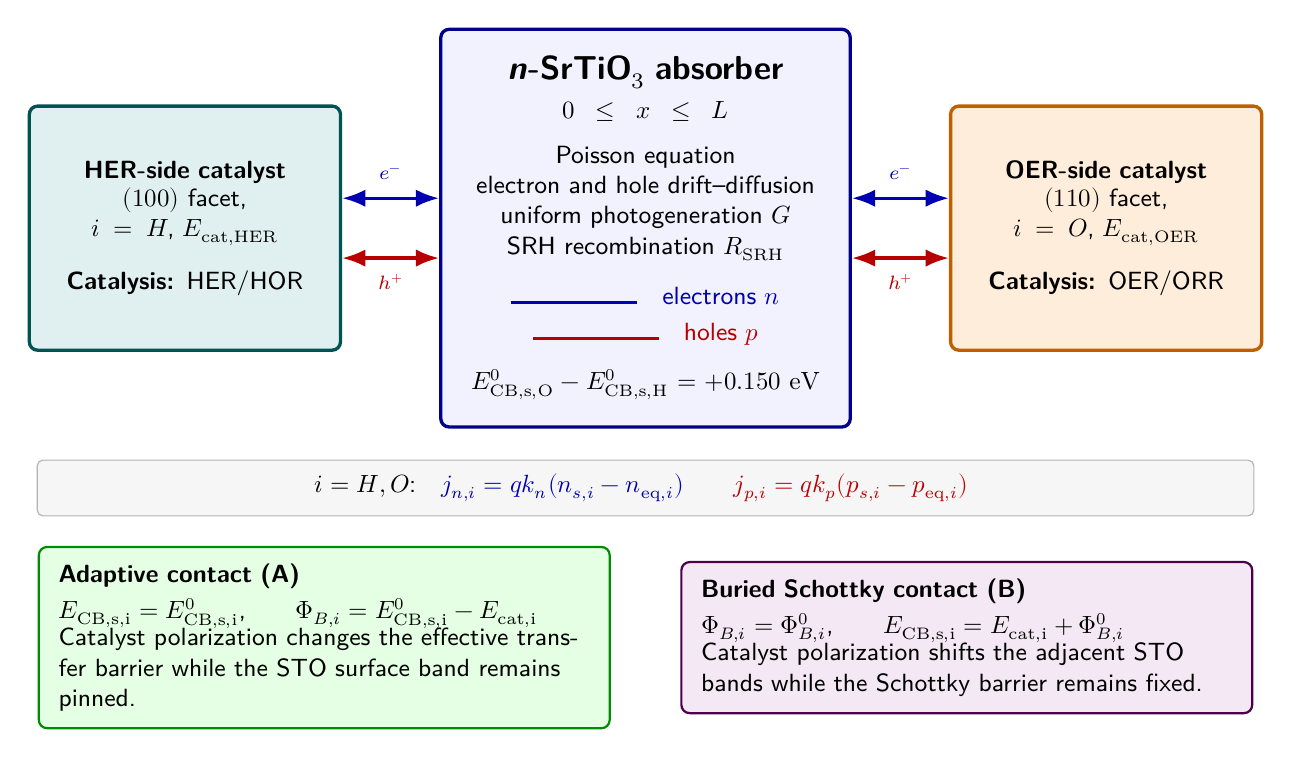
\begin{tikzpicture}[
  x=1cm,y=1cm,
  font=\small\sffamily,
  >=Latex,
  contact/.style={draw,very thick,rounded corners=3pt,align=center,inner sep=5pt},
  transfer/.style={<->,very thick},
  condition/.style={draw,thick,rounded corners=3pt,align=left,inner sep=6pt}
]
\node[contact,fill=teal!12,draw=teal!65!black,minimum width=3.95cm,
      minimum height=3.10cm,text width=3.60cm] (her) at (2.05,6.35) {%
  \textbf{HER-side catalyst}\\[-1pt]
  $(100)$ facet, $i=H$, $E_{\rm cat,HER}$\\[8pt]
  \textbf{Catalysis:} HER/HOR
};

\node[contact,fill=blue!5,draw=blue!55!black,minimum width=5.20cm,
      minimum height=5.05cm,text width=4.70cm] (sto) at (7.90,6.35) {%
  {\large\textbf{\emph{n}-SrTiO$_3$ absorber}}\\[3pt]
  $0\leq x\leq L$\\[5pt]
  Poisson equation\\
  electron and hole drift--diffusion\\
  uniform photogeneration $G$\\
  SRH recombination $R_{\rm SRH}$\\[7pt]
  \textcolor{blue!70!black}{\rule{1.6cm}{1.2pt}\quad electrons $n$}\\[2pt]
  \textcolor{red!72!black}{\rule{1.6cm}{1.2pt}\quad holes $p$}\\[7pt]
  $E_{\rm CB,s,O}^{0}-E_{\rm CB,s,H}^{0}=+0.150~\mathrm{eV}$
};

\node[contact,fill=orange!14,draw=orange!75!black,minimum width=3.95cm,
      minimum height=3.10cm,text width=3.60cm] (oer) at (13.75,6.35) {%
  \textbf{OER-side catalyst}\\[-1pt]
  $(110)$ facet, $i=O$, $E_{\rm cat,OER}$\\[8pt]
  \textbf{Catalysis:} OER/ORR
};

\draw[transfer,blue!70!black] ([yshift=0.38cm]sto.west) -- ([yshift=0.38cm]her.east);
\draw[transfer,red!72!black]  ([yshift=-0.38cm]sto.west) -- ([yshift=-0.38cm]her.east);
\draw[transfer,blue!70!black] ([yshift=0.38cm]sto.east) -- ([yshift=0.38cm]oer.west);
\draw[transfer,red!72!black]  ([yshift=-0.38cm]sto.east) -- ([yshift=-0.38cm]oer.west);

\node[fill=white,inner sep=1pt,font=\scriptsize\bfseries,text=blue!70!black]
  at ($(her.east)!0.5!(sto.west)+(0,0.68)$) {$e^-$};
\node[fill=white,inner sep=1pt,font=\scriptsize\bfseries,text=red!72!black]
  at ($(her.east)!0.5!(sto.west)+(0,-0.68)$) {$h^+$};
\node[fill=white,inner sep=1pt,font=\scriptsize\bfseries,text=blue!70!black]
  at ($(sto.east)!0.5!(oer.west)+(0,0.68)$) {$e^-$};
\node[fill=white,inner sep=1pt,font=\scriptsize\bfseries,text=red!72!black]
  at ($(sto.east)!0.5!(oer.west)+(0,-0.68)$) {$h^+$};

\node[draw=gray!60,fill=gray!7,rounded corners=2pt,align=center,
      minimum width=15.45cm,inner sep=5pt] at (7.90,3.05) {%
  $i=H,O$:\quad
  \textcolor{blue!70!black}{$j_{n,i}=qk_n(n_{s,i}-n_{{\rm eq},i})$}\qquad
  \textcolor{red!72!black}{$j_{p,i}=qk_p(p_{s,i}-p_{{\rm eq},i})$}
};

\node[condition,fill=green!10,draw=green!55!black,minimum width=7.25cm,
      text width=6.75cm] at (3.82,1.15) {%
  \textbf{Adaptive contact (A)}\\[2pt]
  $E_{\rm CB,s,i}=E_{\rm CB,s,i}^{0}$,\qquad
  $\Phi_{B,i}=E_{\rm CB,s,i}^{0}-E_{\rm cat,i}$\\[-1pt]
  Catalyst polarization changes the effective transfer barrier while the STO surface band remains pinned.
};
\node[condition,fill=violet!9,draw=violet!60!black,minimum width=7.25cm,
      text width=6.75cm] at (11.98,1.15) {%
  \textbf{Buried Schottky contact (B)}\\[2pt]
  $\Phi_{B,i}=\Phi_{B,i}^{0}$,\qquad
  $E_{\rm CB,s,i}=E_{\rm cat,i}+\Phi_{B,i}^{0}$\\[-1pt]
  Catalyst polarization shifts the adjacent STO bands while the Schottky barrier remains fixed.
};
\end{tikzpicture}%
}
\caption{\textbf{Spatial model and adaptive/buried contact limits.} A one-dimensional \emph{n}-STO absorber is bounded by an HER-side contact associated with the nominally electron-collecting (100) facet and an OER-side contact associated with the nominally hole-collecting (110) facet. Bidirectional arrows indicate reversible electron and hole exchange. The local interfacial transfer currents $j_{n,i}$ and $j_{p,i}$ are defined as positive for semiconductor-to-catalyst transfer at either interface; their relation to the signed $+x$ semiconductor currents therefore depends on the interface and carrier type, as specified below. The lower panels distinguish the adaptive and buried electrostatic boundary conditions.}

\label{fig:model-framework}
\end{figure}


\subsection{Notation and modeled physical states}

Electronic energies are denoted by $E$ and quoted in eV. Thus $E_{\rm CB}(x)$ and $E_{\rm VB}(x)$ are conduction- and valence-band energies, while $E_{F,n}(x)$, $E_{F,p}(x)$, and $E_{\rm cat,i}$ are the electron and hole quasi-Fermi energies and the catalyst electron electrochemical potential, respectively. Voltages are denoted by $V$; catalyst electrode potentials $V_{\rm cat,i}$ are referenced to RHE. With $q>0$ the elementary charge and the RHE electron-energy reference chosen as $E_{\rm RHE}=0$, the conversion is
\begin{equation}
\boxed{E_{\rm cat,i}=E_{\rm RHE}-qV_{\rm cat,i}.}
\label{eq:energy-potential-map}
\end{equation}
The same conversion applies to band and quasi-Fermi levels expressed on an electrode-potential coordinate. Numerically, $E/\mathrm{eV}=-V/\mathrm{V}$ for this reference. More-negative electrode potentials therefore correspond to higher electron energies, consistent with the energy diagrams of Mills \textit{et al.}\cite{mills2014} Dimensional equations below use energies in joules with SI values of $q$ and $k_B$; reported energies are converted to eV. The band edges obey
\begin{equation}
E_{\rm VB}(x)=E_{\rm CB}(x)-E_g.
\end{equation}
The catalyst-potential separation is
\begin{equation}
\boxed{\Delta V_{\rm cat}=V_{\rm cat,OER}-V_{\rm cat,HER}
=\frac{E_{\rm cat,HER}-E_{\rm cat,OER}}{q}.}
\label{eq:DeltaEcat}
\end{equation}

Three physical states are used. In the \emph{dark equilibrium reference}, photogeneration and electrolyte Faradaic exchange are disabled. The electronically connected solid has one spatially uniform Fermi level,
\begin{equation}
E_{\rm cat,HER}=E_{\rm cat,OER}=E_F,\qquad J_n=J_p=0.
\end{equation}
The common value is set to $E_F=0$ eV, corresponding to a common electrode potential of 0 V versus RHE, when the dark band bending is reported. In an \emph{illuminated catalyst-off state}, photogeneration is active but electrolyte reactions are disabled, so
\begin{equation}
J_{\rm sem}=J_n+J_p=0.
\label{eq:catalyst-off}
\end{equation}
In a \emph{finite-current OWS state}, HER and OER kinetics are active and the two catalyst charge balances determine $E_{\rm cat,HER}$, $E_{\rm cat,OER}$, and the operating current.

\subsection{Semiconductor transport model}

The STO occupies $0\leq x\leq L$, with the HER contact at $x=0$ and the OER contact at $x=L$. Nondegenerate carrier statistics are used:
\begin{align}
n(x)&=N_C\exp\!\left[-\frac{E_{\rm CB}(x)-E_{F,n}(x)}{k_BT}\right],\\
p(x)&=N_V\exp\!\left[-\frac{E_{F,p}(x)-E_{\rm VB}(x)}{k_BT}\right].
\end{align}
The thermal voltage is $V_T=k_BT/q$. The electron density-of-states mass is $m_n^*=1.8m_e$, consistent with reduced single-crystal STO,\cite{ahrens2007} while $m_p^*=3.0m_e$ is a representative valence-band density-of-states parameter. These values give $N_C=6.00\times10^{19}$ cm$^{-3}$ and $N_V=1.29\times10^{20}$ cm$^{-3}$ at 298.15 K.

For uniformly ionized donors $N_D$, the conduction-band energy satisfies Poisson's equation. With electrostatic potential $\phi$ (in V) and $E_{\rm CB}=\mathrm{constant}-q\phi$,
\begin{equation}
\boxed{\frac{d^2E_{\rm CB}}{dx^2}=\frac{q^2}{\epsilon_0\epsilon_r}\left(p-n+N_D\right).}
\label{eq:poisson}
\end{equation}
Electron and hole currents are written in quasi-Fermi-energy form,
\begin{equation}
\boxed{J_n=\mu_n n\frac{dE_{F,n}}{dx},}\qquad
\boxed{J_p=\mu_p p\frac{dE_{F,p}}{dx},}
\label{eq:dd}
\end{equation}
which is equivalent to the standard drift--diffusion equations with the Einstein relation. Steady-state continuity requires
\begin{equation}
\boxed{\frac{dJ_n}{dx}=q(R-G),}\qquad
\boxed{\frac{dJ_p}{dx}=q(G-R),}
\label{eq:continuity}
\end{equation}
so $J_n+J_p$ is spatially constant. Bulk recombination is described by mid-gap Shockley--Read--Hall kinetics,\cite{shockleyread1952,hall1952}
\begin{equation}
\boxed{R_{\rm SRH}=\frac{np-n_i^2}{\tau_p(n+n_i)+\tau_n(p+n_i)}.}
\label{eq:srh}
\end{equation}
The baseline lifetimes are idealized transport parameters. They control the quantitative bulk-recombination loss and operating current. The distinction between adaptive and buried architectures arises from the contact boundary conditions and is not sensitive to the particulary lifetime chosen.

Generation is uniform in space so that optical absorption does not introduce a left--right asymmetry. Its magnitude reproduces the total Beer--Lambert absorbed photon flux:
\begin{equation}
G=\frac{I_0(1-e^{-\alpha L})}{(hc/\lambda)L},\qquad
J_{\rm gen}=qGL.
\label{eq:generation}
\end{equation}
For $I_0=10$ mW cm$^{-2}$, $\lambda=365$ nm, $\alpha=10^6$ m$^{-1}$, and $L=1~\mu$m, $G=1.16\times10^{20}$ cm$^{-3}$ s$^{-1}$ and $J_{\rm gen}=1.86$ mA cm$^{-2}$.

\begin{table}[p]
\centering
\caption{\textbf{Baseline parameters for the spatial adaptive-junction model.} The final column distinguishes literature- or experiment-motivated quantities from representative model choices.}
\label{tab:modelparams}
\scriptsize
\begin{tabular}{@{}p{0.16\textwidth}p{0.17\textwidth}p{0.27\textwidth}p{0.31\textwidth}@{}}
\toprule
Parameter & Baseline value & Model role & Basis \\
\midrule
$T$ & 298.15 K & temperature & operating condition \\
$L$ & 1.0 $\mu$m & baseline STO thickness & model geometry; varied in Fig.~\ref{fig:thickness} \\
$N_D$ & $10^{18}$ cm$^{-3}$ & uniform n-type doping & representative model input \\
$\epsilon_r$ & 300 & STO dielectric constant & room-temperature bulk STO\cite{neville1972} \\
$E_g$ & 3.20 eV & STO band gap & near the measured indirect gap\cite{vanbenthem2001} \\
$m_n^*,m_p^*$ & $1.8m_e,3.0m_e$ & effective DOS masses & measured electron DOS mass;\cite{ahrens2007} representative hole DOS mass \\
$\mu_n,\mu_p$ & 5, 0.1 cm$^2$ V$^{-1}$ s$^{-1}$ & electron/hole mobilities & representative first-order transport inputs \\
$\tau_n,\tau_p$ & 100 $\mu$s & SRH lifetimes & idealized model choice \\
$\lambda$ & 365 nm & excitation wavelength & simulated operating condition \\
$I_0$ & 10 mW cm$^{-2}$ & baseline intensity & simulated operating condition \\
$\alpha$ & $10^6$ m$^{-1}$ & absorption coefficient & representative near-edge scale; $\alpha^{-1}=1~\mu$m\cite{cohen1968} \\
$V_{\rm bb,H}^0$ & 0.85 V & native HER-side depletion bending & representative depletion scale; paired with the measured facet difference\cite{assavachin2024} \\
$V_{\rm bb,O}^0$ & 1.00 V & native OER-side depletion bending & representative depletion scale; $0.15$-V difference constrained by experiment\cite{assavachin2024} \\
$k_n=k_p$ & 10 m s$^{-1}$ & reversible interfacial transfer coefficient & symmetric model choice in the Mills boundary law\cite{mills2014} \\
$V_{\rm HER}^{\rm eq}$ & 0 V vs RHE & HER/HOR equilibrium & thermodynamic reference \\
$V_{\rm OER}^{\rm eq}$ & 1.229 V vs RHE & OER/ORR equilibrium & thermodynamic reference \\
$j_{0,H},j_{0,O}$ & $10^{-6},10^{-12}$ A cm$^{-2}$ & exchange currents & illustrative catalyst kinetic parameters \\
$b_H,b_O$ & 0.100, 0.040 V dec$^{-1}$ & anodic/cathodic Tafel slopes & illustrative catalyst kinetic parameters \\
$j_{\rm lim,HOR},j_{\rm lim,ORR}$ & 50 $\mu$A cm$^{-2}$ & gas-consuming reverse limits & reverse-branch model choice \\
\bottomrule
\end{tabular}
\end{table}

The implementation uses the conduction-band reference $E_{\rm CB}^{\rm ref}=+0.400$ eV, corresponding to $-0.400$ V versus RHE. Pan \textit{et al.} used $-0.40$ V versus RHE for the SrTiO$_3$ conduction-band edge in water, while Han \textit{et al.} reported $-0.30$ V versus RHE for undoped SrTiO$_3$ and values near $-0.39$ to $-0.41$ V versus RHE after Mg incorporation.\cite{pan2020,han2017}

\subsection{Native facet asymmetry and contact boundary conditions}

The native facet input is motivated by the preferential reduction and oxidation behavior of STO (100) and (110) surfaces.\cite{takata2020,assavachin2024} Assavachin \textit{et al.} measured facet-dependent flat-band potentials differing by approximately 0.13 V and estimated a doping-corrected barrier difference up to approximately 0.16 eV.\cite{assavachin2024} The baseline therefore uses depletion bendings of 0.85 V on the HER/(100) side and 1.00 V on the OER/(110) side. The depletion-bending voltage is defined by $qV_{\rm bb,i}=E_{\rm CB,s,i}-E_{\rm CB,bulk}$. We define the mean and differential native bendings as
\begin{align}
\overline V_{\rm bb}^{0}&=\frac{V_{\rm bb,H}^{0}+V_{\rm bb,O}^{0}}{2}=0.925~\mathrm V,\\
\Delta V_{\rm bb}^{0}&=V_{\rm bb,O}^{0}-V_{\rm bb,H}^{0}=0.150~\mathrm V.
\label{eq:mean-differential-bending}
\end{align}
The mean controls the overall degree of depletion at the two surfaces. The differential term breaks left--right symmetry and sets the preferred direction of carrier collection.

With the dark Fermi level chosen as $E_F=0$ eV, the neutral-bulk conduction-band/Fermi-level separation is
\begin{equation}
\Delta E_C=k_BT\ln\!\left(\frac{N_C}{n_0}\right)=0.105~\mathrm{eV}.
\end{equation}
The pinned surface conduction-band positions are
\begin{equation}
E_{\rm CB,s,H}^0\approx+0.955~\mathrm{eV},\qquad
E_{\rm CB,s,O}^0\approx+1.105~\mathrm{eV},
\end{equation}
so
\begin{equation}
\boxed{E_{\rm CB,s,O}^0-E_{\rm CB,s,H}^0=q\Delta V_{\rm bb}^0=+0.150~\mathrm{eV}.}
\label{eq:nativeasymmetry}
\end{equation}
Larger positive depletion bending raises the surface conduction-band energy.

Carrier transfer is represented by the reversible constant-density-of-states boundary rate expressions proposed and used by Mills \textit{et al.}\cite{mills2014} At contact $i$, the carrier populations in local detailed balance with $E_{\rm cat,i}$ are
\begin{align}
n_{{\rm eq},i}&=N_C\exp\!\left[-\frac{E_{\rm CB,s,i}-E_{\rm cat,i}}{k_BT}\right],\\
p_{{\rm eq},i}&=N_V\exp\!\left[-\frac{E_{\rm cat,i}-E_{\rm VB,s,i}}{k_BT}\right].
\end{align}
The signed net transfer currents, positive from semiconductor to catalyst, are
\begin{align}
\boxed{j_{n,i}=qk_n\left(n_{s,i}-n_{{\rm eq},i}\right),}\\
\boxed{j_{p,i}=qk_p\left(p_{s,i}-p_{{\rm eq},i}\right).}
\label{eq:carriertransfer}
\end{align}
Each is the difference between semiconductor-to-catalyst and catalyst-to-semiconductor one-way currents; for example, $j_{n,i}^{\rm S\rightarrow C}=qk_n n_{s,i}$ and $j_{n,i}^{\rm C\rightarrow S}=qk_n n_{{\rm eq},i}$. These $j_{n,i}$ and $j_{p,i}$ are local outward-transfer scalars, whereas $J_n$ and $J_p$ in Eq.~\ref{eq:dd} are conventional semiconductor current densities referenced to the global $+x$ direction. The boundary signs are therefore
\begin{equation}
J_n(0)=j_{n,H},\qquad J_p(0)=-j_{p,H},\qquad
J_n(L)=-j_{n,O},\qquad J_p(L)=j_{p,O}.
\label{eq:transfer-signs}
\end{equation}
The opposite signs for electrons and holes follow from the opposite signs of their charge; the opposite signs at $x=0$ and $x=L$ follow from the outward surface normals.

Here $k_n$ and $k_p$ are first-order heterogeneous interfacial transfer coefficients. Their dimensions are velocity because multiplying $k$ by a volumetric carrier concentration gives an areal number flux. The baseline uses
\begin{equation}
\boxed{k_n=k_p=10~\mathrm{m~s^{-1}}}
\end{equation}
at both contacts. Hamann, Gstrein, Brunschwig, and Lewis measured second-order outer-sphere electron-transfer rate constants near optimum driving force of approximately $0.5$--$1\times10^{-16}$ cm$^4$ s$^{-1}$ at n-ZnO/water interfaces.\cite{hamann2005free,hamann2005reorg,hamann2006ph} At 5 mM dissolved acceptor, these values correspond to effective first-order transfer coefficients of approximately 1.5--3 m s$^{-1}$. The 10 m s$^{-1}$ baseline is therefore deliberately fast but chemically comparable in scale. It is not fitted to STO.\@ The equality $k_n=k_p$ prevents carrier selectivity from being imposed through unequal microscopic transfer coefficients; selectivity instead emerges from the electrostatic boundary conditions and carrier populations.

At an adaptive contact, ionic, dipolar, or chemical compensation permits the catalyst electron electrochemical potential to move while the STO surface band remains pinned:
\begin{equation}
\boxed{E_{\rm CB,s,i}=E_{\rm CB,s,i}^{0},}\qquad
\boxed{\Phi_{B,i}=E_{\rm CB,s,i}^{0}-E_{\rm cat,i}.}
\label{eq:adaptivebc}
\end{equation}
Here $\Phi_B$ is the electron barrier energy, quoted in eV. At a buried contact, the physical Schottky barrier remains fixed. The barriers matched to the native dark bendings are
\begin{equation}
\Phi_{B,H}^{0}=0.955~\mathrm{eV},\qquad
\Phi_{B,O}^{0}=1.105~\mathrm{eV},
\end{equation}
and the boundary obeys
\begin{equation}
\boxed{E_{\rm CB,s,i}=E_{\rm cat,i}+\Phi_{B,i}^{0},}\qquad
\boxed{E_{\rm CB,s,i}-E_{\rm cat,i}=\Phi_{B,i}^{0}.}
\label{eq:buriedbc}
\end{equation}
The catalyst/electrolyte interface may still charge and polarize, but that shift appears one-for-one in the adjacent semiconductor bands rather than changing the buried Schottky barrier.

The adaptive catalyst reservoir is treated as locally screened and does not introduce a separate long-range space-charge field in the STO.\@ For an oxide/oxyhydroxide catalyst, this model represents redox-coupled ion insertion. For Pt/H, it represents the net potential-dependent response of interfacial H species, adsorbates, and the double layer ions which may partially penetrate the Pt/STO interface which is likely hydrated. This representations however does not imply formation of a bulk Pt hydride.

\subsection{Catalyst kinetics and steady-state charge balance}

The catalyst overpotentials are
\begin{equation}
\eta_H=V_{\rm cat,HER}-V_{\rm HER}^{\rm eq}=V_{\rm cat,HER},\qquad
\eta_O=V_{\rm cat,OER}-V_{\rm OER}^{\rm eq}=V_{\rm cat,OER}-1.229~\mathrm V.
\end{equation}
Equivalently, $q\eta_i=E_{\rm redox,i}-E_{\rm cat,i}$, where $E_{\rm redox,H}=0$ eV and $E_{\rm redox,O}=-1.229$ eV on the chosen energy reference. Positive current is anodic: $j_H>0$ is HOR, $j_H<0$ is HER, $j_O>0$ is OER, and $j_O<0$ is ORR.\@ The kinetic numerator is the standard reversible Butler--Volmer expression,\cite{bardfaulkner2001}
\begin{equation}
j_i^{\rm BV}=j_{0,i}\left[
\exp\!\left(\frac{\alpha_{a,i}F\eta_i}{RT}\right)
-\exp\!\left(-\frac{\alpha_{c,i}F\eta_i}{RT}\right)
\right]
=j_{0,i}\left[10^{\eta_i/b_{a,i}}-10^{-\eta_i/b_{c,i}}\right],
\label{eq:butler-volmer}
\end{equation}
where $b_{a,i}=2.303RT/(\alpha_{a,i}F)$ and $b_{c,i}=2.303RT/(\alpha_{c,i}F)$. The model uses the symmetric phenomenological choice $b_{a,i}=b_{c,i}=b_i$. An algebraic limiting-current correction is applied only to the gas-consuming HOR and ORR branches:
\begin{align}
f_H^+&=10^{\eta_H/b_H}, & f_H^-&=10^{-\eta_H/b_H},\\
f_O^+&=10^{\eta_O/b_O}, & f_O^-&=10^{-\eta_O/b_O},
\end{align}
\begin{align}
\boxed{j_H=j_{0,H}\frac{f_H^+-f_H^-}{1+(j_{0,H}/j_{\rm lim,HOR})f_H^+},}\\
\boxed{j_O=j_{0,O}\frac{f_O^+-f_O^-}{1+(j_{0,O}/j_{\rm lim,ORR})f_O^-}.}
\label{eq:faradaic}
\end{align}
The reverse limiting currents do not affect the forward AA and BA OWS operating points reported below.

With reactions active, steady catalyst charge balance requires
\begin{equation}
\boxed{J_{\rm sem}+j_H=0,}\qquad
\boxed{-J_{\rm sem}+j_O=0.}
\label{eq:catalyst-balance}
\end{equation}
Here $J_{\rm sem}\equiv J_n+J_p$ is the spatially constant conventional current density within the semiconductor, defined as positive in the $+x$ direction from the HER-side contact toward the OER-side contact. For forward OWS, electron collection at the HER side and hole collection at the OER side both contribute to $J_{\rm sem}>0$. Thus
\begin{equation}
\boxed{J_{\rm OWS}=J_{\rm sem}=j_O=-j_H>0.}
\label{eq:owsbalance}
\end{equation}


\subsection{Numerical solutions}

Equations~\ref{eq:poisson}--\ref{eq:continuity} are solved as a nonlinear boundary-value problem using SciPy's residual-controlled collocation solver \texttt{solve\_bvp}.\cite{kierzenka2001} The coordinate is scaled by $s=x/L$, and logarithmic carrier densities preserve positivity through depleted regions. The solver evaluates the algebraically equivalent voltage-coordinate equations using $-E/q$ relative to the chosen energy zero; publication energies are obtained by Eq.~\ref{eq:energy-potential-map}. The initial mesh is cosine-clustered toward both contacts and is adaptively refined by the collocation solver. Continuation in illumination, catalyst potential, or current supplies initial guesses only; each reported endpoint satisfies the original steady equations. Total-current constancy, both catalyst charge balances, the integrated current balance, and the collocation residual are checked for every reported state.

Table~\ref{tab:architectures} separates the no catalyst/solution current open-circuit voltage condition calculation from finite-current catalytic operation calculation. For architectures containing ideal adaptive catalyst junctions, disabling electrolyte reactions does not provide two independent catalyst charge-balance equations. The AA, AB, and BA entries are therefore the selected zero-current states used in the main article to compare differential polarization; they are not unique conventional photovoltaic open-circuit operating points as the particle itself is electrically floating. Their selection does not enter the finite-current AA or BA calculations. For BB, the catalyst-off voltage is $(\Phi_{B,O}^0-\Phi_{B,H}^0)/q=0.150$ V.

\begin{table}[ht]
\centering
\caption{\textbf{Adaptive and buried architectures at 10 mW cm$^{-2}$.} Selected catalyst-off separations reproduce the states shown in the main article. Finite-current entries are reported only for architectures that support forward OWS with the stated kinetic model.}
\label{tab:architectures}
\small
\begin{tabular}{@{}lcccc@{}}
\toprule
Architecture & AA & AB & BA & BB \\
\midrule
HER-side contact & adaptive & adaptive & buried & buried \\
OER-side contact & adaptive & buried & adaptive & buried \\
Selected catalyst-off $\Delta V_{\rm cat}$ (V) & 2.72 & 0.696 & 2.17 & 0.150 \\
Exceeds 1.229 V? & yes & no & yes & no \\
Forward OWS in model? & yes & no & yes & no \\
$J_{\rm OWS}$ (mA cm$^{-2}$) & 0.945 & --- & 0.0304 & --- \\
$E_{\rm cat,HER}$ (eV) & $+0.298$ & --- & $+0.148$ & --- \\
$E_{\rm cat,OER}$ (eV) & $-1.59$ & --- & $-1.53$ & --- \\
Operating $\Delta V_{\rm cat}$ (V) & 1.89 & --- & 1.68 & --- \\
\bottomrule
\end{tabular}
\end{table}

BB retains only the native 0.150-V contact asymmetry, far below the 1.229-V reversible OWS requirement. AB reaches a larger selected catalyst-off separation but remains subthreshold. Neither architecture can sustain forward OWS under the stated conditions. In the presence of both product gases, reversible electrochemical loading is therefore directed toward H$_2$/O$_2$ recombination; the corresponding reverse rate depends on gas activities and transport parameters and is not used in the architecture comparison.

For forward operation, the interfacial contact-recombination current is defined as the total opposite-carrier transfer at the two contacts. With the present sign convention,
\begin{equation}
\boxed{J_{\rm contact}=-J_p(0)-J_n(L)\geq 0,}
\label{eq:contact-recombination}
\end{equation}
where $-J_p(0)$ is undesired hole transfer at the HER contact and $-J_n(L)$ is undesired electron transfer at the OER contact. These fluxes neutralize the complementary catalyst charge and therefore constitute contact-mediated recombination, also described as interfacial counterflow. The integrated bulk loss is
\begin{equation}
J_{\rm SRH}=q\int_0^L R_{\rm SRH}\,dx,
\end{equation}
and the steady-state current balance is
\begin{equation}
\boxed{J_{\rm gen}=J_{\rm OWS}+J_{\rm contact}+J_{\rm SRH}.}
\label{eq:current-balance}
\end{equation}

The fully adaptive AA state gives
\begin{equation}
\boxed{J_{\rm OWS}^{AA}=0.945~\mathrm{mA~cm^{-2}},}\qquad
\boxed{E_{\rm cat,HER}=+0.298~\mathrm{eV},\quad E_{\rm cat,OER}=-1.59~\mathrm{eV},}
\end{equation}
with
\begin{equation}
\boxed{\Delta V_{\rm cat}^{AA}=1.89~\mathrm V.}
\end{equation}


Both surface bands remain pinned, so the native surface-band energy difference remains exactly $+0.150$ eV as the catalyst potentials separate. The steady-state current balance is
\begin{equation}
1.86=0.945+0.912+0.00307
\qquad \mathrm{mA~cm^{-2}},
\label{eq:aa-balance}
\end{equation}
where the terms are useful OWS current, contact recombination, and bulk SRH recombination. Contact recombination is the dominant loss because the baseline intentionally uses equal electron and hole transfer coefficients.

The half-adaptive BA state also supports forward OWS, but to a much smaller degree:
\begin{equation}
\boxed{J_{\rm OWS}^{BA}=0.0304~\mathrm{mA~cm^{-2}},}\qquad
\boxed{E_{\rm cat,HER}=+0.148~\mathrm{eV},\quad E_{\rm cat,OER}=-1.53~\mathrm{eV},}
\end{equation}
with
\begin{equation}
\boxed{\Delta V_{\rm cat}^{BA}=1.68~\mathrm V.}
\end{equation}
The buried HER contact shifts the HER-side surface band to approximately $+1.104$ eV, while the adaptive OER-side band remains pinned near $+1.105$ eV. Only 1.67 meV of the original 150-meV directional surface-band energy difference remains. Cathodic polarization of the HER catalyst raises its electron energy and the adjacent STO bands together at fixed barrier height. The fixed-barrier condition is $\Phi_{B,H}=E_{C,s,H}-E_{\rm cat,H}=0.955$ eV. Local HER depletion remains, with
\[
V_{\rm bb,H}=\frac{E_{C,s,H}-E_{C,\rm bulk}}{q}=0.309~\mathrm V,
\]
compared with 0.850 V in the dark reference. The electrically floating semiconductor bulk also shifts under operation: relative to the dark reference, $E_{C,s,H}$ rises by 0.148 eV whereas $E_{C,\rm bulk}$ rises by 0.690 eV. The larger bulk shift reduces the local band bending by 0.541 V while the buried Schottky barrier remains fixed. The fixed barrier therefore coexists with reduced local depletion in the floating semiconductor. Because the OER-side band remains pinned, the HER-side surface shift simultaneously brings the two surface band edges into near coincidence and removes the left--right electrostatic asymmetry that directed carrier collection. The resulting loss of directional selectivity produces strong contact recombination and a much smaller OWS current:
\begin{equation}
1.86=0.0304+1.83+0.00327
\qquad \mathrm{mA~cm^{-2}}.
\label{eq:ba-balance}
\end{equation}

\begin{figure}[htbp]
\centering

\includegraphics[width=0.98\textwidth]{figures/Figure_S16_AA_BA_operating_profiles.pdf}
\caption{\textbf{Finite-current AA and BA OWS states.} The ordinate is electron energy in eV relative to $E_{\rm RHE}=0$, increasing upward. Solid curves are the STO band edges, dashed curves are the electron and hole quasi-Fermi levels, short horizontal segments are the catalyst electron electrochemical potentials, and dotted horizontal lines are the solution redox references. (a) In AA, both surface band edges remain pinned, preserving the native 0.150-eV surface-band energy difference while the catalyst potentials separate. (b) In BA, cathodic polarization of the buried HER catalyst raises its electron energy and the adjacent STO bands at fixed barrier height. Local HER depletion remains but is reduced relative to the dark reference because the floating semiconductor bulk shifts more strongly, while the directional surface-band energy difference between the contacts falls to 1.67 meV. The centered boxes report $J_{\rm gen}=J_{\rm OWS}+J_{\rm contact}+J_{\rm SRH}$ in mA cm$^{-2}$.}
\label{fig:operating-profiles}
\end{figure}
\clearpage


\subsection{Sensitivity to native facet asymmetry}

The native junction is parameterized by the mean bending $\overline V_{\rm bb}^{0}$ and differential bending $\Delta V_{\rm bb}^{0}$ defined in Eq.~\ref{eq:mean-differential-bending}. In the AA limit, both surface band edges are pinned. For the AA case, the imposed differential bending is therefore retained during catalyst polarization rather than being expended to generate $\Delta V_{\rm cat}$ as in the BB or mixed cases. With otherwise identical adaptive contacts, $\Delta V_{\rm bb}^{0}=0$ gives no preferred direction and no net OWS current in the symmetric model. At the baseline mean bending, increasing $\Delta V_{\rm bb}^{0}$ from 0.05 to 0.10, 0.15, 0.20, and 0.30 V increases $J_{\rm OWS}$ from 0.704 to 0.907, 0.945, 0.956, and 0.969 mA cm$^{-2}$, respectively. Thus a 50-mV native asymmetry already produces approximately three quarters of the baseline current, and the response progressively saturates. At fixed $\Delta V_{\rm bb}^{0}=0.15$ V, varying $\overline V_{\rm bb}^{0}$ from 0.70 to 1.15 V hardly changes the current from 0.944 to 0.945 mA cm$^{-2}$.

\begin{figure}[ht]
\centering

\includegraphics[width=0.98\textwidth]{figures/Figure_S17_native_asymmetry_sensitivity.pdf}
\caption{\textbf{Sensitivity to native facet band bending.} (a) AA OWS current versus differential native bending for several values of the mean native bending. Differential bending establishes directionality, with most of the increase occurring below approximately 0.15 V. (b) At fixed $\Delta V_{\rm bb}^{0}=0.15$ V, the current depends only weakly on the mean native bending. The vertical dotted lines mark the baseline values.}
\label{fig:native-bending-sensitivity}
\end{figure}
\clearpage

\subsection{Sensitivity to interfacial transfer coefficient and illumination}

The common first-order semiconductor--catalyst transfer coefficient was varied from 0.1 to 1000 m s$^{-1}$ while maintaining $k_n=k_p$ at both contacts. The AA OWS current changes only from 0.954 to 0.941 mA cm$^{-2}$ and $\Delta V_{\rm cat}$ remains essentially constant. Increasing a nonselective common coefficient accelerates desired and undesired transfer together, producing a modest increase in contact recombination.

The 365-nm intensity was varied from 1 to 30 mW cm$^{-2}$. $J_{\rm OWS}$ increases from 0.0944 to 2.84 mA cm$^{-2}$ while $J_{\rm OWS}/J_{\rm gen}$ remains approximately 50.7--50.9\%. The operating catalyst separation increases from 1.75 to 1.95 V because larger HER and OER overpotentials are required at higher current.

\begin{figure}[htbp]
\centering

\includegraphics[width=0.98\textwidth]{figures/Figure_S18_transfer_intensity_sensitivity.pdf}
\caption{\textbf{Sensitivity to the common interfacial transfer coefficient and illumination intensity.} (a,b) Varying the same electron and hole transfer coefficient at both contacts over four decades has little effect on AA OWS current or catalyst separation; faster nonselective transfer modestly increases contact recombination. (c,d) OWS current scales approximately linearly with absorbed photon-equivalent current, while the finite-current catalyst separation increases to supply the larger catalytic overpotentials. Panels (b,d) show the catalyst energy separation $E_{\rm cat,HER}-E_{\rm cat,OER}=q\Delta V_{\rm cat}$ and the central quasi-Fermi splitting $E_{F,n}-E_{F,p}$, both in eV.}
\label{fig:rate-intensity}
\end{figure}
\clearpage

\subsection{Sensitivity to absorber thickness}
\label{sec:thickness}

The fully adaptive AA calculation was repeated from $L=0.01$ to 10 $\mu$m with all other parameters fixed. Thickness changes two quantities simultaneously: the total absorbed photon flux and the distance over which carriers are transported. At each thickness, the generation rate remains spatially uniform, while its magnitude is chosen so that
\begin{equation}
J_{\rm gen}(L)=q\frac{I_0}{hc/\lambda}\left(1-e^{-\alpha L}\right),
\qquad
G(L)=\frac{J_{\rm gen}(L)}{qL}.
\label{eq:thickness-generation}
\end{equation}
The generated current is partitioned according to Eq.~\ref{eq:current-balance}.


Three regimes are evident. At small $L$, incomplete absorption limits $J_{\rm gen}$ and therefore $J_{\rm OWS}$. As $L$ approaches and exceeds the absorption length $\alpha^{-1}=1~\mu$m, the absorbed photon current rises and the OWS current increases. At larger $L$, absorption approaches saturation while carrier transport distances and bulk SRH loss increase, causing the OWS current to decline. For the stated absorption coefficient, mobilities, and lifetimes, the current has a broad maximum near 4 $\mu$m. This thickness is specific to the selected parameter set and is not a universal optimum particle size. The finite-current catalyst separation remains above the reversible OWS requirement throughout the simulated range.

\begin{table}[ht]
\centering
\caption{\textbf{Representative AA thickness-sweep operating points.} Current densities are in mA cm$^{-2}$.}
\label{tab:thickness}
\scriptsize
\begin{tabular}{@{}rrrrrr@{}}
\toprule
$L$ ($\mu$m) & $J_{\rm OWS}$ & $\Delta V_{\rm cat}$ (V) & $J_{\rm gen}$ & $J_{\rm contact}$ & $J_{\rm SRH}$ \\
\midrule
0.010 & 0.0288 & 1.67 & 0.0293 & 0.000498 & $6.88\times10^{-9}$ \\
0.100 & 0.214 & 1.80 & 0.280 & 0.0664 & $3.41\times10^{-6}$ \\
0.316 & 0.425 & 1.84 & 0.798 & 0.373 & $3.39\times10^{-5}$ \\
1.00 & 0.945 & 1.89 & 1.86 & 0.912 & 0.00307 \\
3.98 & 1.39 & 1.91 & 2.89 & 1.38 & 0.120 \\
10.0 & 1.14 & 1.90 & 2.94 & 1.15 & 0.653 \\
\bottomrule
\end{tabular}
\end{table}


\begin{figure}[htbp]
\centering

\includegraphics[width=0.98\textwidth]{figures/Figure_S19_AA_thickness_sensitivity.pdf}
\caption{\textbf{AA sensitivity to absorber thickness.} (a) Absorbed photon-equivalent current, useful OWS current, interfacial contact-recombination current, and integrated bulk SRH loss. These terms satisfy Eq.~\ref{eq:current-balance}. (b) Finite-current catalyst-potential separation. The vertical dotted line marks the baseline thickness and the absorption length, $L=\alpha^{-1}=1~\mu$m; the horizontal dashed line marks the 1.229-V reversible OWS requirement.}
\label{fig:thickness}
\end{figure}

\clearpage

\subsection{Physical interpretation, assumptions, and reproducibility}

 The 0.150-V native STO facet asymmetry is sufficient to direct complementary carrier collection but cannot itself provide the OWS voltage through two fixed Schottky contacts. BB therefore produces only 0.150 V, and AB remains subthreshold for driving OWS. 
 
 BA can drive OWS because the adaptive OER contact can polarize substantially without shifting its surface band. At the buried HER contact, cathodic catalyst polarization raises the catalyst electron energy and the adjacent STO bands one-for-one at fixed Schottky barrier. Because the floating STO bulk shifts more strongly, the local HER-side band bending decreases even though the barrier height is unchanged. The surface-band energy difference between the HER and OER sides is nevertheless nearly eliminated, strongly suppressing directional collection. AA preserves the native asymmetry at both surfaces while the catalyst electron electrochemical potentials separate, giving the much larger OWS current.

The model is intentionally idealized. STO permittivity is field independent; carrier statistics are nondegenerate; native facet electrostatics are represented by pinned surface band edges rather than an explicit distribution of surface states and Helmholtz capacitance; adaptive catalyst reservoirs are locally and perfectly screened; electrolyte transport and double-layer structure are not explicitly modeled; $k_n=k_p$ omits material-specific microscopic transfer selectivity; photogeneration is uniform; and the HER/OER kinetics are illustrative reversible Butler--Volmer/Tafel relations. The buried controls omit tunneling, thermionic-field emission, interface leakage,  breakdown, and other high-field processes. The adaptive-catalyst junction approximation omits finite ionic transport, finite redox capacity, and explicit charging dynamics. The Pt/H contact is represented by the same effective redox-responsive reservoir abstraction as the oxide OER contact despite their different microscopic chemistry. 

The one-dimensional geometry omits catalyst shape, facet edges, lateral transport, and current crowding. These assumptions affect quantitative currents and optimal dimensions. However, these modelling assumptions do not change the boundary-condition distinction tested here. Catalyst polarization preserves the STO surface band at an adaptive contact and shifts it at a buried contact.

The model implementation, numerical outputs, figure-generation routines, and validation tests are archived at
\url{https://github.com/ajkaufman25/NatureCatalysis-CooperativeAdaptiveJunctions-1D-2026}.


\clearpage
\setcounter{figure}{19}


\begin{figure}[p]
\centering
\includegraphics[width=\textwidth,height=0.86\textheight,keepaspectratio]{figures/Figure_S23_dark_illuminated_CV.pdf}
\caption{\textbf{Dark and illuminated cyclic voltammograms.} a) bare \textit{n}-STO b) CoO$_x$-deposited \textit{n}-STO with cobalt reduction occurring at $\sim -1.1$~V vs.\ Hg/HgO c) Pt-deposited \textit{n}-STO d) Pt- and CoO$_x$-deposited \textit{n}-STO with cobalt reduction occurring at $\sim -1.1$~V vs.\ Hg/HgO. These curves highlight differences in the electrochemical behavior of the four samples under dark and illuminated conditions. Relative to the bare semiconductor, the Pt- and/or CoO$_x$-deposited samples exhibit lower photocurrents because the deposited materials block portions of the photoelectrochemically active semiconductor surface.}
\label{fig:dark_light_cv}
\end{figure}



\clearpage

\begin{figure}[p]
\centering
\includegraphics[width=0.90\textwidth,height=0.70\textheight,keepaspectratio]{figures/Figure_S24_reductive_discharge.pdf}
\caption{\textbf{Illuminated electrochemical reductive discharge following photocharging.} Reductive-discharge cyclic voltammograms of bare, Pt-deposited, CoO$_x$-deposited, and Pt/CoO$_x$-deposited samples. a) Discharge response at $100~\mathrm{mV\,s^{-1}}$ following 60~s of photocharging. b) Baseline-subtracted discharge response following 60~s of photocharging. The background reductive current was calculated by averaging cycles 8--10 and subsequently subtracted from cycles 1 and 2. c) Discharge response at $100~\mathrm{mV\,s^{-1}}$ following 10~s of photocharging. d) Baseline-subtracted discharge response following 10~s of photocharging. The larger reductive-discharge response of the Pt/CoO$_x$-deposited sample shown in (b) is consistent with complementary electron- and hole-selective sites promoting greater spatial charge separation and enabling greater accumulation of photogenerated charge.}
\label{fig:reductive_discharge}
\end{figure}
\clearpage

\begin{figure}[p]
\centering
\includegraphics[width=0.90\textwidth,height=0.70\textheight,keepaspectratio]{figures/Figure_S25_dark_discharge.pdf}
\caption{\textbf{Dark-discharge cyclic voltammograms before photocharging.} Before any illuminated photocharging experiments, the samples were electrochemically discharged to reduce oxidized surface species by cycling the applied potential between $-1.2$ and $-0.8$~V three times in the dark.}
\label{fig:dark_discharge_prephotocharging}
\end{figure}
\clearpage


\subsection*{Additional discussion of the dimensionless barrier response}
\addcontentsline{toc}{subsection}{Additional discussion of the dimensionless barrier response}

The CoO$_x$ | \textit{n}-STO junction exhibits a dimensionless apparent barrier response
\begin{equation}
S_{\rm b}\equiv-\frac{d\Phi_{\rm b}}{dE_{\rm cat}}
=\frac{1}{q}\frac{d\Phi_{\rm b}}{dV_{\rm cat}}
=1.4\pm0.3,
\label{eq:barrier-response}
\end{equation}
determined from three independent experiments (Figure~3). The minus sign follows from $E_{\rm cat}=E_{\rm RHE}-qV_{\rm cat}$; $S_{\rm b}=1$ for an ideally pinned adaptive contact and $S_{\rm b}=0$ for a fixed-barrier buried contact. Here,
$\Phi_{\mathrm{b}}$ is extracted from fits to dark majority-carrier
current--voltage measurements and therefore represents an effective barrier
governing interfacial transport. Within the ideal electrostatic description
considered here, a one-volt change in catalyst potential produces at most a
one-electronvolt change in barrier energy. The fitted response above unity
consequently warrants consideration of transport contributions that are not
explicitly resolved by this description.

The fitting model describes the interfacial current--voltage response using
two adjustable parameters: the barrier height, $\Phi_{\mathrm{b}}$, and the
diode ideality factor, $n$. Changes in current arising from processes outside
this parameterization can therefore be incorporated into either or both
fitted quantities. For example, oxidation of CoO$_x$ may alter the density
of electronic states available for electron transfer or the intrinsic
semiconductor--catalyst transfer rate. If these changes decrease the
transport prefactor, a fit that assumes a constant prefactor can attribute
the resulting current suppression to an increased barrier height. The
apparent barrier would then contain both electrostatic and kinetic
contributions, potentially yielding
$S_{\rm b}>1$
without a corresponding electrostatic response above unity.

As shown in Figure~\ref{fig:coox-ideality}, the fitted ideality factor varies with
$V_{\rm cat}$ for CoO$_x$ junctions on both (100)- and (110)-oriented
\textit{n}-STO. This potential dependence indicates that catalyst polarization
changes the shape of the interfacial current--voltage response, in addition
to the apparent barrier extracted from its magnitude. The junction response
therefore cannot be described solely by a changing barrier in an otherwise
invariant ideal-diode characteristic. Redox charging, ion insertion,
interfacial charging, and changes in surface-state occupation provide
possible microscopic contributions to this behavior. Although these
processes are consistent with an adaptive interface, their individual
contributions cannot be distinguished from the present fits. We therefore
interpret the measured slope as an effective junction response rather than
a direct measurement of electrostatic barrier modulation above unity.

The one-dimensional model does not use the measured CoO$_x$ slope as an
input or require a response above unity. Instead, adaptation is represented
through the interfacial electrostatic boundary conditions. At an adaptive
contact, the STO surface band energy remains pinned while the catalyst
electron electrochemical potential shifts, changing the effective transfer
barrier. At a buried contact, the barrier remains fixed while the adjacent
STO surface bands shift with catalyst potential. The simulations thus
examine how the two interfaces interact through the shared absorber
independently of the precise fitted CoO$_x$ slope. The proposed mechanism
relies on complementary changes in the Pt- and CoO$_x$-side junctions,
rather than on interpreting the apparent response above unity as
electrostatic amplification.

\begin{figure}[ht]
\centering
\includegraphics[width=0.96\textwidth]{figures/Figure_S26_nvsEcat_AuCo_Compare.pdf}
\caption{Ideality factor for CoO$x$ | n-STO junctions as a function of the catalyst potential $V_{\rm cat}$ showing a degree of non-ideal behavior that may be responsible in part for the dimensionless barrier response $S_{\rm b}>1$.}
\label{fig:coox-ideality}
\end{figure} 



\clearpage
\phantomsection
\addcontentsline{toc}{section}{References}
\begin{thebibliography}{99}

\bibitem{teeter2019}
G. Teeter, S. P. Harvey, C. L. Perkins, K. Ramanathan, and I. L. Repins,
``Comparative operando XPS studies of quasi-Fermi level splitting and open-circuit voltage in CZTSe/CdS and CIGS/CdS junctions and device structures,''
\textit{J. Vac. Sci. Technol. A} \textbf{37} (2019).

\bibitem{lin2014}
F. Lin and S. W. Boettcher,
``Adaptive semiconductor/electrocatalyst junctions in water-splitting photoanodes,''
\textit{Nature Materials} \textbf{13}, 81--86 (2014). doi:10.1038/nmat3811.

\bibitem{mills2014}
T. J. Mills, F. Lin, and S. W. Boettcher,
``Theory and simulations of electrocatalyst-coated semiconductor electrodes for solar water splitting,''
\textit{Phys. Rev. Lett.} \textbf{112}, 148304 (2014). doi:10.1103/PhysRevLett.112.148304.

\bibitem{nellist2016}
M. R. Nellist, F. A. L. Laskowski, F. Lin, T. J. Mills, and S. W. Boettcher,
``Semiconductor--Electrocatalyst Interfaces: Theory, Experiment, and Applications in Photoelectrochemical Water Splitting,''
\textit{Acc. Chem. Res.} \textbf{49}, 733--740 (2016). doi:10.1021/acs.accounts.6b00001.

\bibitem{shockleyread1952}
W. Shockley and W. T. Read, Jr.,
``Statistics of the Recombinations of Holes and Electrons,''
\textit{Phys. Rev.} \textbf{87}, 835--842 (1952). doi:10.1103/PhysRev.87.835.

\bibitem{hall1952}
R. N. Hall,
``Electron-Hole Recombination in Germanium,''
\textit{Phys. Rev.} \textbf{87}, 387 (1952). doi:10.1103/PhysRev.87.387.

\bibitem{assavachin2024}
S. Assavachin, C. Xiao, K. Becker, and F. E. Osterloh,
``Facets control charge separation during photoelectrochemical water oxidation with strontium titanate (SrTiO$_3$) single crystals,''
\textit{Energy Environ. Sci.} \textbf{17}, 3493--3502 (2024). doi:10.1039/D3EE04308H.

\bibitem{takata2020}
T. Takata, J. Jiang, Y. Sakata, M. Nakabayashi, N. Shibata, V. Nandal, K. Seki, T. Hisatomi, and K. Domen,
``Photocatalytic water splitting with a quantum efficiency of almost unity,''
\textit{Nature} \textbf{581}, 411--414 (2020). doi:10.1038/s41586-020-2278-9.

\bibitem{pan2020}
Z. Pan, R. Yanagi, Q. Wang, X. Shen, Q. Zhu, Y. Xue, J. A. R\"ohr, T. Hisatomi, K. Domen, and S. Hu,
``Mutually-dependent kinetics and energetics of photocatalyst/co-catalyst/two-redox liquid junctions,''
\textit{Energy Environ. Sci.} \textbf{13}, 162--173 (2020). doi:10.1039/C9EE02910A.

\bibitem{han2017}
K. Han, Y.-C. Lin, C.-M. Yang, R. Jong, G. Mul, and B. Mei,
``Promoting Photocatalytic Overall Water Splitting by Controlled Magnesium Incorporation in SrTiO$_3$ Photocatalysts,''
\textit{ChemSusChem} \textbf{10}, 4510--4516 (2017). doi:10.1002/cssc.201701794.

\bibitem{kierzenka2001}
J. Kierzenka and L. F. Shampine,
``A BVP Solver Based on Residual Control and the MATLAB PSE,''
\textit{ACM Trans. Math. Softw.} \textbf{27}, 299--316 (2001). doi:10.1145/502800.502801.

\bibitem{neville1972}
R. C. Neville, B. Hoeneisen, and C. A. Mead,
``Permittivity of Strontium Titanate,''
\textit{J. Appl. Phys.} \textbf{43}, 2124--2131 (1972). doi:10.1063/1.1661463.

\bibitem{vanbenthem2001}
K. van Benthem, C. Els\"asser, and R. H. French,
``Bulk electronic structure of SrTiO$_3$: Experiment and theory,''
\textit{J. Appl. Phys.} \textbf{90}, 6156--6164 (2001). doi:10.1063/1.1415766.

\bibitem{ahrens2007}
M. Ahrens, R. Merkle, B. Rahmati, and J. Maier,
``Effective masses of electrons in n-type SrTiO$_3$ determined from low-temperature specific heat capacities,''
\textit{Physica B} \textbf{393}, 239--248 (2007). doi:10.1016/j.physb.2007.01.008.

\bibitem{cohen1968}
M. I. Cohen and R. F. Blunt,
``Optical Properties of SrTiO$_3$ in the Region of the Absorption Edge,''
\textit{Phys. Rev.} \textbf{168}, 929--932 (1968). doi:10.1103/PhysRev.168.929.

\bibitem{bardfaulkner2001}
A. J. Bard and L. R. Faulkner,
\textit{Electrochemical Methods: Fundamentals and Applications}, 2nd ed. (Wiley, New York, 2001).


\bibitem{hamann2005free}
T. W. Hamann, F. Gstrein, B. S. Brunschwig, and N. S. Lewis,
``Measurement of the Free-Energy Dependence of Interfacial Charge-Transfer Rate Constants Using ZnO/H$_2$O Semiconductor/Liquid Contacts,''
\textit{J. Am. Chem. Soc.} \textbf{127}, 7815--7824 (2005). doi:10.1021/ja0436188.

\bibitem{hamann2005reorg}
T. W. Hamann, F. Gstrein, B. S. Brunschwig, and N. S. Lewis,
``Measurement of the Dependence of Interfacial Charge-Transfer Rate Constants on Reorganization Energy at n-ZnO/H$_2$O Interfaces,''
\textit{J. Am. Chem. Soc.} \textbf{127}, 13949--13954 (2005). doi:10.1021/ja0515452.

\bibitem{hamann2006ph}
T. W. Hamann, F. Gstrein, B. S. Brunschwig, and N. S. Lewis,
``Measurement of the Driving Force Dependence of Interfacial Charge-Transfer Rate Constants through pH Changes at n-ZnO/H$_2$O Interfaces,''
\textit{Chem. Phys.} \textbf{326}, 15--23 (2006). doi:10.1016/j.chemphys.2006.02.027.

\end{thebibliography}

\end{document}
